% Options for packages loaded elsewhere
\PassOptionsToPackage{unicode}{hyperref}
\PassOptionsToPackage{hyphens}{url}
\PassOptionsToPackage{dvipsnames,svgnames,x11names}{xcolor}
%
\documentclass[
  10pt,
]{article}
\usepackage{amsmath,amssymb}
\usepackage{iftex}
\ifPDFTeX
  \usepackage[T1]{fontenc}
  \usepackage[utf8]{inputenc}
  \usepackage{textcomp} % provide euro and other symbols
\else % if luatex or xetex
  \usepackage{unicode-math} % this also loads fontspec
  \defaultfontfeatures{Scale=MatchLowercase}
  \defaultfontfeatures[\rmfamily]{Ligatures=TeX,Scale=1}
\fi
\usepackage{lmodern}
\ifPDFTeX\else
  % xetex/luatex font selection
  \setmainfont[]{DejaVu Serif}
  \setmonofont[]{DejaVu Sans Mono}
\fi
% Use upquote if available, for straight quotes in verbatim environments
\IfFileExists{upquote.sty}{\usepackage{upquote}}{}
\IfFileExists{microtype.sty}{% use microtype if available
  \usepackage[]{microtype}
  \UseMicrotypeSet[protrusion]{basicmath} % disable protrusion for tt fonts
}{}
\makeatletter
\@ifundefined{KOMAClassName}{% if non-KOMA class
  \IfFileExists{parskip.sty}{%
    \usepackage{parskip}
  }{% else
    \setlength{\parindent}{0pt}
    \setlength{\parskip}{6pt plus 2pt minus 1pt}}
}{% if KOMA class
  \KOMAoptions{parskip=half}}
\makeatother
\usepackage{xcolor}
\usepackage[margin=18mm]{geometry}
\usepackage{graphicx}
\makeatletter
\def\maxwidth{\ifdim\Gin@nat@width>\linewidth\linewidth\else\Gin@nat@width\fi}
\def\maxheight{\ifdim\Gin@nat@height>\textheight\textheight\else\Gin@nat@height\fi}
\makeatother
% Scale images if necessary, so that they will not overflow the page
% margins by default, and it is still possible to overwrite the defaults
% using explicit options in \includegraphics[width, height, ...]{}
\setkeys{Gin}{width=\maxwidth,height=\maxheight,keepaspectratio}
% Set default figure placement to htbp
\makeatletter
\def\fps@figure{htbp}
\makeatother
\setlength{\emergencystretch}{3em} % prevent overfull lines
\providecommand{\tightlist}{%
  \setlength{\itemsep}{0pt}\setlength{\parskip}{0pt}}
\setcounter{secnumdepth}{-\maxdimen} % remove section numbering
\ifLuaTeX
  \usepackage{selnolig}  % disable illegal ligatures
\fi
\usepackage{bookmark}
\IfFileExists{xurl.sty}{\usepackage{xurl}}{} % add URL line breaks if available
\urlstyle{same}
\hypersetup{
  colorlinks=true,
  linkcolor={Maroon},
  filecolor={Maroon},
  citecolor={Blue},
  urlcolor={Blue},
  pdfcreator={LaTeX via pandoc}}

\author{}
\date{}

\begin{document}

\section{Twist torsion yields a degree-17 source
endomorphism}\label{twist-torsion-yields-a-degree-17-source-endomorphism}

The same public p827 fixture now has an explicit endomorphism of the
source curve, built from twist torsion:

\[
\alpha=(\pi+[1])/[7],\qquad
(1-\alpha)\alpha=\alpha(1-\alpha)=[17],\qquad
\alpha^2-\alpha+[17]=0.
\]

These are \textbf{generic rational-function identities}, checked in
native Rust and independently in PARI. The Frobenius identity is checked
as {[}7{]}α=π+{[}1{]}, including x\^{}827 and y·f(x)\^{}413; division
notation above denotes this certified endomorphism. It is not scalar
inversion only on a finite group. This supplies a further explicit
twist-derived connection to the source generator arithmetic. Standard
isogeny/endomorphism theory is prior art; no novel index-calculus
speedup or NIST result is established.

On E:y²=x³+x+15 over F827, group order823, G=(2,5), Q=37G, the map acts
as \(\alpha(P)=[353]P\) for every rational P. Hence α(Q)=k·α(G) whenever
Q=kG. The generator image is(189,620), the target image is(451,814), and
scalar415 inverts this action modulo823. All823 points, including
infinity, are checked; all822 wrong-scalar354 controls are rejected. No
unknown logarithm is recovered by evaluating a known scalar action.

The d2 twist is Y²=X³+4X+120, order833=C7×C119. Starting from the
already verified maximal-order point H=(2,386), the
fixed{[}7{]}H=(345,743) has order17. Its anti-Frobenius embedding
supplies the eight paired x-roots of the kernel. Normalized Vélu gives
the intermediate curve y²=x³+31x+77. The fixed coordinate isomorphism
(x,y)↦(49x,343y) returns to the source and gives α. The sign and scale
were specified before the output; no alternative kernel was selected.

On all833 embedded twist-rational points, α has kernel17 and image49
killed by7. This is consistent with {[}7{]}α=π+{[}1{]} and the original
odd-component Frobenius separation. It does not transport the order823
DLP into the rational twist group. The scalar353 has multiplicative
order274 modulo823, independently verified. Evaluating or folding such
orbits requires charged work; an orbit length alone establishes no
computational gain. The morphism has degree17.

\begin{figure}
\centering
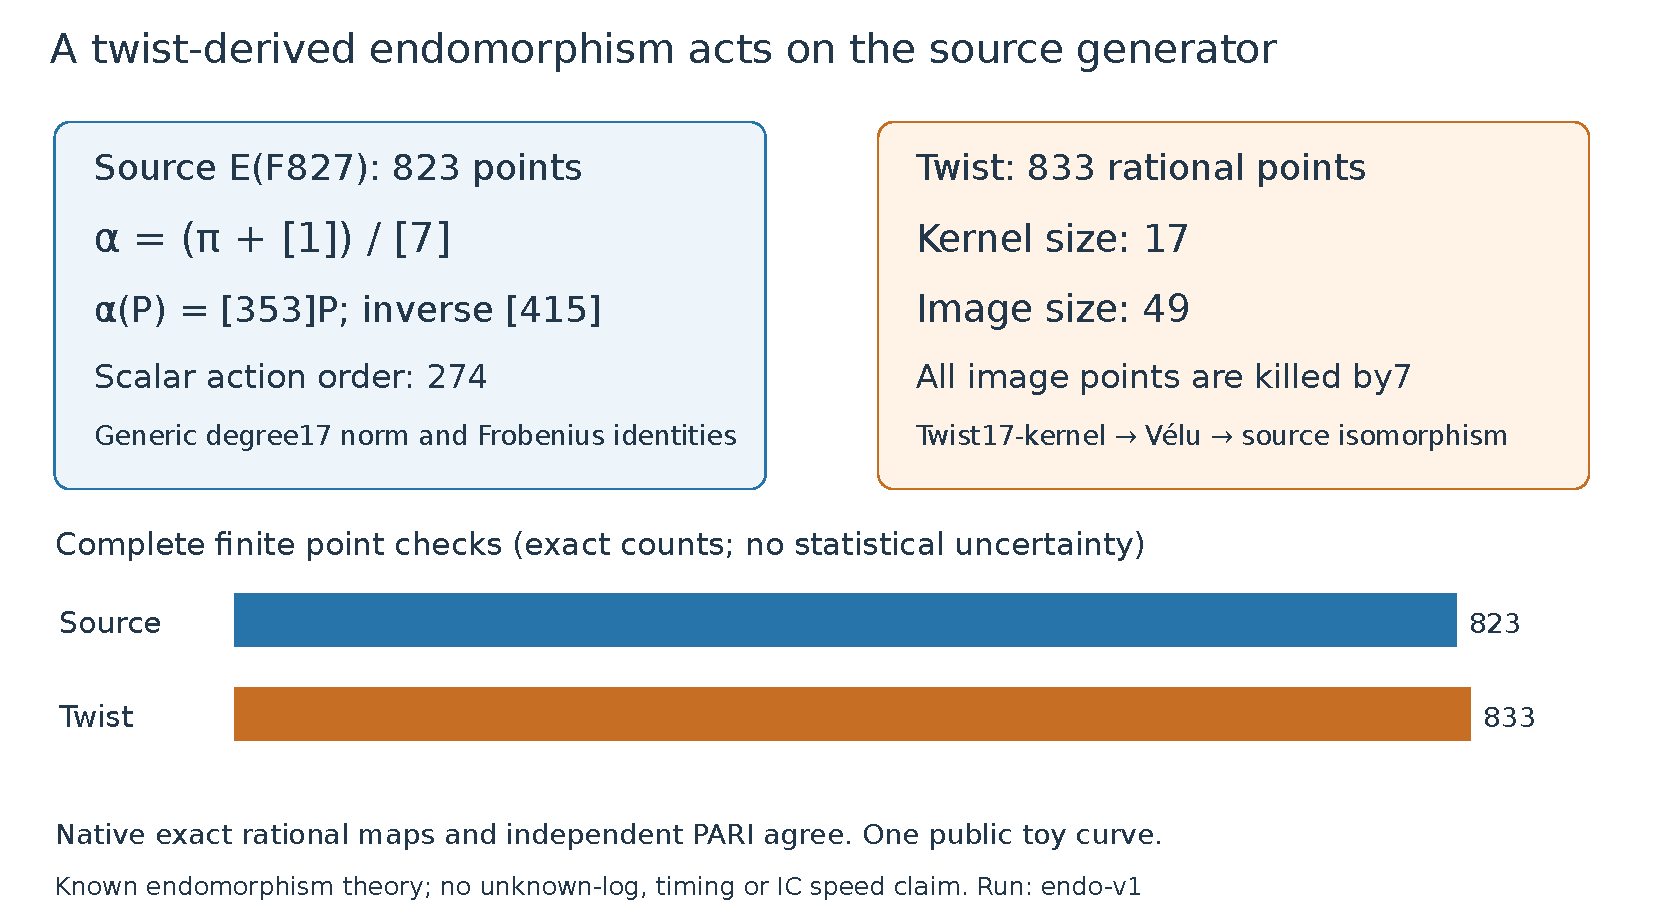
\includegraphics{CONNECTION.pdf}
\caption{Verified endomorphism, source action and twist image}
\end{figure}

The native producer constructs rational functions (X(x),yS(x)), the
conjugate id−α and independent generic{[}7{]}/{[}17{]} maps. It checks
both degree17 norm compositions and the Frobenius identity exactly, then
the complete finite source/twist sets. GP independently builds
\texttt{ellisogeny}, reconstructs generic group arithmetic, checks the
same identities, and evaluates the conjugated map
(X,Y)↦(2R(X/2),Y·S(X/2)) on the rational twist. Native and GP agree;
strict admission allows only the exact declared GP stack-size warning.
No scientific stage fails or reaches its cap. Two actual complete-panel
executions pass; their unified protocol/export/file binding has zero
findings.

Source c12290db\allowbreak{}2fd94b4a\allowbreak{}929b2e05\allowbreak{}86ff8973\allowbreak{}dd8079a1; protocol
1bfb4a24\allowbreak{}bf342ec3\allowbreak{}70dfaa59\allowbreak{}b861449f\allowbreak{}d7b59c42\allowbreak{}2effd85d\allowbreak{}ef05139f\allowbreak{}47df5523.
Source/binaries/spec were frozen, committed and checkpointed before
data. Bounds300s each,4GiB,CPU0,one thread,L0 managed Xeon
Platinum8573C/KVM. The documented EKS access/image fallback applies.
Operational timestamps are unadmitted; no paid resource or IAM change.
The v8 arithmetic/map prefix is a byte-preserved versioned snapshot;
older frozen source and data stay unchanged.

Three conditional Lean declarations pass fresh native axiom audit:

\begin{itemize}
\tightlist
\item
  \texttt{TwistEndomorphism.norm\_polynomial} assumes a commutative
  ring, a+b=1 and ba=17.
\item
  \texttt{frobenius\_polynomial} derives the trace5/norm827 polynomial
  from a²−a+17=0.
\item
  \texttt{inverse\_scalar} proves415·353 acts as identity on
  an823-torsion additive group.
\end{itemize}

Foundations are propext and Quot.sound, with no sorry/custom
axiom/trusted native evaluation. Concrete curve groups, rational maps
and the endomorphism ring bridge are \textbf{not formalized}. The
discriminant−67 is that of the checked quadratic polynomial; no separate
class-polynomial or complete volcano census was run in this experiment.

Literature reviewed before implementation: Sutherland, MIT18.783
Fall2025 Lecture5 Theorems5.11/5.15 and Lecture13
Theorems13.6/13.8/proof; the repository isogeny-loop report and atlas
GLV/GLS/isogeny-loop lead. These sources separate known-scalar
arithmetic from unknown-log solving. A public small fixture with this
structure is not evidence that NIST P-curves have it.

\href{../../execution-v10/README.md}{Reproduction, exact models, ordered
route and raw verification} retain the generator-bound EC1 UIDs, map
artifact hashes, complete scripts, receipts and deterministic Setec
archive. No benchmark/leaderboard row moves. Existing performance graphs
stay unchanged; this exact connection figure is new. The remaining
experiments must price map discovery/evaluation and useful relation
solving on identical tasks. Original full campaigns, calibrated IC/rho
comparison and independent-host replay remain open.

\end{document}
